\documentclass[10pt, a5paper]{article}
\usepackage{pdfpages}
\usepackage{parallel}
\usepackage[T2A]{fontenc}
\usepackage{ucs}
\usepackage[utf8x]{inputenc}
\usepackage[polish,english,russian]{babel}
\usepackage{hyperref}
\usepackage{rotating}
\usepackage[inner=2cm,top=1.8cm,outer=2cm,bottom=2.3cm,nohead]{geometry}
\usepackage{listings}
\usepackage{graphicx}
\usepackage{wrapfig}
\usepackage{longtable}
\usepackage{indentfirst}
\usepackage{array}
\newcolumntype{P}[1]{>{\raggedright\arraybackslash}p{#1}}
\frenchspacing
\usepackage{fixltx2e} %text sub- and superscripts
\usepackage{icomma} % коскі ў матэматычным рэжыме
\PreloadUnicodePage{4}

\newcommand{\longpage}{\enlargethispage{\baselineskip}}
\newcommand{\shortpage}{\enlargethispage{-\baselineskip}}

\def\switchlang#1{\expandafter\csname switchlang#1\endcsname}
\def\switchlangbe{
\let\saverefname=\refname%
\def\refname{Літаратура}%
\def\figurename{Іл.}%
}
\def\switchlangen{
\let\saverefname=\refname%
\def\refname{References}%
\def\figurename{Fig.}%
}
\def\switchlangru{
\let\saverefname=\refname%
\let\savefigurename=\figurename%
\def\refname{Литература}%
\def\figurename{Рис.}%
}

\hyphenation{admi-ni-stra-tive}
\hyphenation{ex-pe-ri-ence}
\hyphenation{fle-xi-bi-li-ty}
\hyphenation{Py-thon}
\hyphenation{ma-the-ma-ti-cal}
\hyphenation{re-ported}
\hyphenation{imp-le-menta-tions}
\hyphenation{pro-vides}
\hyphenation{en-gi-neering}
\hyphenation{com-pa-ti-bi-li-ty}
\hyphenation{im-pos-sible}
\hyphenation{desk-top}
\hyphenation{elec-tro-nic}
\hyphenation{com-pa-ny}
\hyphenation{de-ve-lop-ment}
\hyphenation{de-ve-loping}
\hyphenation{de-ve-lop}
\hyphenation{da-ta-ba-se}
\hyphenation{plat-forms}
\hyphenation{or-ga-ni-za-tion}
\hyphenation{pro-gramming}
\hyphenation{in-stru-ments}
\hyphenation{Li-nux}
\hyphenation{sour-ce}
\hyphenation{en-vi-ron-ment}
\hyphenation{Te-le-pathy}
\hyphenation{Li-nux-ov-ka}
\hyphenation{Open-BSD}
\hyphenation{Free-BSD}
\hyphenation{men-ti-on-ed}
\hyphenation{app-li-ca-tion}

\def\progref!#1!{\texttt{#1}}
\renewcommand{\arraystretch}{2} %Іначай формулы ў матрыцы зліпаюцца з лініямі
\usepackage{array}

\def\interview #1 (#2), #3, #4, #5\par{

\section[#1, #3, #4]{#1 -- #3, #4}
\def\qname{LVEE}
\def\aname{#1}
\def\q ##1\par{{\noindent \bf \qname: ##1 }\par}
\def\a{{\noindent \bf \aname: } \def\qname{L}\def\aname{#2}}
}

\def\interview* #1 (#2), #3, #4, #5\par{

\section*{#1\\{\small\rm #3, #4. #5}}

\def\qname{LVEE}
\def\aname{#1}
\def\q ##1\par{{\noindent \bf \qname: ##1 }\par}
\def\a{{\noindent \bf \aname: } \def\qname{L}\def\aname{#2}}
}

\switchlang{ru}
\begin{document}
\title{Создание СХД  с томами «тонкой» настройки на базе дистрибутива Linux}
\author{Александр Клыга, Minsk, Belarus\footnote{\url{alex_kls@mail.ru}, \url{https://lvee.org/en/abstracts/295}}}
\maketitle
\begin{abstract}
The concept creating a thin provisioning of data storage on based distribution Linux. The ``Thin provisioning'' is a popular creation technology for the data storage. The concept of ``thin provisioning'' is based on ``over-allocation'' or ``over-subscription'' mechanism of dynamically allocated data blocks in a two-level model data storage. On the first level a thin pool is formed which includes the ``data pool'' and ``meta pool''. The second level consists of virtual volumes for the user space. The full size of virtual volumes can be several times large than the capacity of the thin pool. In the Linux distribution the ``Device mapper'' module exists acting as a provider of a thin volumes data storage. You can use the \verb!dmsetup! utility or ``Logical Volume Management 2'' (LVM2) to create and manage the thin provisioning data storage pool and the virtual volumes.
\end{abstract}
\subsection*{Описание, модель хранения данных, основные переменные, пример расчета для СХД с томами \linebreak «тонкой» настройки на базе дистрибутива Linux}
 
Тома с «тонкой» настройкой \cite{bib1} или «подготовкой» (thin provi\-sioning) это виртуальная абстракция устройства хранения данных с заранее определенными параметрами, но имеющим изначально относительно небольшой размер и поддерживающим технологию динамического распределения блоков для хранения данных из общего хранилища.

Они широко применяются в системах хранения данных (СХД) и виртуализации для эффективного использования доступного дискового пространства между пользователями ресурсов с учетом их потребностей.

Данное решение базируется на концепции избыточного распределения, и  разработанных на ее основе технологий и механизмов для создания СХД с использованием виртуальной абстракции \linebreak устройства (файл или блочное устройство).

При этом, формат файла, как виртуальной абстракции устройства  хранения данных, содержит в себе полную структуру и содержимое сходную с форматом жёсткого диска, а его размер может быть фиксированным (определено максимальное его значение) или динамическим (размер файла изменяется по мере его заполнения данными до максимального заданного значения).

Если в качестве виртуальной абстракции используется блочное устройство, то, может использоваться одноуровневая или двухуровневая модель  хранения данных.

При одноуровневой модели создается виртуальное блочное \linebreak устройство большой емкости, при начальной инициализации содержащий небольшое количество блоков для хранения данных, дополнительные блоки добавляются из хранилища по мере необходимости (максимальное количество блоков которое может быт добавлено в устройство определяется переменной).

При двухуровневой модели (рисунок \ref{02:klyga:fig1}) создаются две виртуальные абстракции: общий пул хранения данных и виртуальные логические тома для пользователей.

\begin{center}
\begin{figure}[h!]
  \centering
  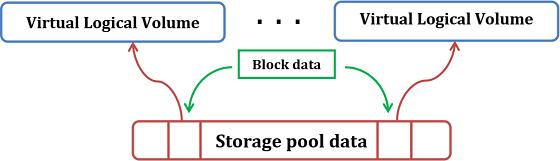
\includegraphics[width=8cm]{02_klyga_fig1}
  \caption{Двухуровневая модель}
  \label{02:klyga:fig1}
\end{figure}
\end{center} 

Распределением блоков для хранения данных из общего пула между виртуальными логическими томами управляет программа-менеджер. В случае необходимости новые блоки для хранения данных добавляются в общий пул, и в автоматическом режиме распределяются между виртуальными логическими томами, исключая необходимость проводить дополнительные манипуляции с ними (например, изменения размера файловой системы). При этом реальный размер каждого виртуального логического томам может превосходить суммарный объем общего пула хранения данных.

В ядре Linux абстракции виртуальных блочных устройств реализуются с помощью модуля «Device mapper» \cite{bib2}, а начиная с версии ядра 3.2 в него добавлена поддержка динамического выделения места в хранилище данных (thin provisioning) с возможностью реализации двухуровневой модели хранения данных.

При создании СХД с использование томов с «тонкой» настройкой (thin provisioning) \cite{bib3} на базе дистрибутива Linux необходимо учитывать версию ядра, возможности поддержки требуемого функционала с помощью дополнительных модулей, и  расширения общего пула хранения данных с учетом возрастающих потребностей.

Типовая структурная схема включает в себя два основных компонента: пул устройств (или том с ``тонкой'' настройкой thin pool) объединяющий вместе том метаданных (meta pool) и том данных (data pool)  и виртуальные тома (virtual volume) для пространства пользователя. В случае использования менеджера логических томов LVM2 \cite{bib4}, создание пулов томов с ``тонкой'' настройкой (thin pool) осуществляется в пределах одной Volume Group (VG) (рисунок \ref{02:klyga:fig2}).

\begin{center}
\begin{figure}[h!]
  \centering
  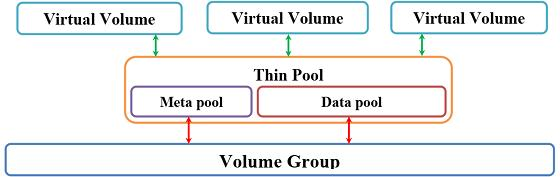
\includegraphics[width=9cm]{02_klyga_fig2}
  \caption{Типовая структурная схема СХД с томами ``тонкой'' настройки}
  \label{02:klyga:fig2}
\end{figure}
\end{center} 

При этом несмотря на это ограничение использование LVM2 более предпочтительно так как позволяет использовать дополнительные возможности:

\begin{itemize}
  \item подключение внешнего хранилища, доступного в режиме только для чтения в качестве основы для создания типовых LVM-разделов, при котором все обращения на чтение не изменённых данных прозрачно транслируются к базовому эталонному хранилищу, а все изменённые или новые данные обрабатываются в отдельном слое в режиме чтения-записи;
  \item поддержку динамической агрегации метаданных при помощи демона lvmetad;
  \item поддержку технологии LVM Cache для общих пулов хранения данных;
  \item работы со снапшотами.
\end{itemize}

Перед созданием СХД необходимо определить  параметры каждого виртуального тома, их суммарный общий объем (переменная \verb!$data_dev_size_max!), текущий доступный объем  для тома данных (переменная \verb!$data_dev_size!), возможность использования дополнительных накопителей для тома с метаданными (включая возможность резервирования), выбрать программу-менеджер для управления и используя формулы приведенные ниже определить значения ключевых переменных, при этом, для утилиты \verb!dmsetup! модуля «Device mapper» все значения указываются в количестве блоков, для LVM2 в байтах или других представлениях единиц измерений.

\subsection*{Размер виртуальных томов (virtual volume)}

Размер виртуальных томов (virtual volume) для пространства пользователей определяет администратор на основании технического задания или иных предпочтений, однако, при этом суммарный размер виртуальных томов не должен превышать предельно допустимые физические параметры системы  хранения данных в целом, в случае необходимости  должна быть реализована возможность их расширения с учетом возрастающих потребностей.

\subsection*{Размер фрагмента выделения (chunk size)}

\verb!$data_block_size=$dev_min_block_size * $count_block!, \\ где
\verb!$dev_min_block_size! – минимальный размер блока данных на устройстве, как правило, это значение равно 512 байт.
\verb!$count_block! – количество блоков данных которые можно использовать при раздаче, как правило от 128 до 2097152 для обычных томов данных, для сложной структуры 128, для снапшотов от 8 до 1048576.

\subsection*{Размер тома с метаданными}

\noindent{\small\verb!$metadata_dev_size = 48 * $data_dev_size_max / $data_block_size!}, \\где
\verb!$data_dev_size_max!  –  полный размер тома данных;\\
\verb!$data_block_size! – размер фрагмента выделения. 
При этом необходимо учитывать, что размер тома для хранения метаданных не может быть меньше 2Мб, и больше 16Гб, рекомендуемое значение по умолчанию 1Гб. Если по итогам расчетов размер тома для хранения метаданных превышает значение 16Гб, рекомендуется создавать несколько пулов хранения данных.

К размещению метаданных тонких томов стоит относится аккуратно, так  как, если данное пространство будет исчерпано, то пул будет выдавать ошибки ввода-вывода до тех пор, пока пул не будет переведен в автономный режим, и не будет выполнено восстановление для устранения потенциальных несоответствий. Поэтому, рекомендуется для пространства метаданных использовать отдельное выделенное устройство или несколько устройств с возможностью резервирования (например, объединить их в raid 1), а для повышения производительности использовать твердотельные накопители.

\subsection*{Определение значения переменной \\ \$low\_water\_mark}

{\small\verb!$low_water_mark = $count_block_sign_error * $data_block_size!},
\\ \verb!$count_block_sign_error! — значение количества свободных блоков в пуле данных при достижении которого выдать сигнал об исчерпании места;
\verb!$data_block_size! — текущее значение размера блока распределения.

Значение переменной \verb!$count_block_sign_error! определяется \linebreak системным администратором исходя из размера пула и критичности его оперативного расширения. 

Значение переменной \verb!$low_water_mark! используется для генерации однократного сигнала предупреждения при достижении низкого уровня свободного места в пуле хранения данных.

После выполнения расчета и анализа результатов, если необходимо провести корректировку значения \verb!$data_dev_size!, определить устройства для хранения данных и метаданных и выполнить первичную сборку и настройку СХД.

Пример расчета:

Условие:
Необходимо создать хранилище данных для 100 виртуальных машин с томами размером по 50GB для каждой, при наличии физического дискового пространства в 200GB и одного накопителя sdd емкостью 128GB.

\begin{enumerate}
  \item Определим значение переменной \verb!$data_dev_size_max!:\\
\verb!$data_dev_size_max!=100*50*1073741824=5 368 709 120 000 \linebreak байт
  \item Определим значение переменной \verb!$data_dev_size!, установив его в 98\% от максимально возможного (\textbf{рекомендовано}): 
\verb!$data_dev_size!=(200*1073741824)*0.98=210 453 397 504 байт
  \item Определим размер фрагмента выделения значением по умолчанию в 128 блоков по 512 байт:\\
 \verb!$data_block_size! = 128 * 512 =65 536 байт
  \item Определим размер тома для хранения метаданных:\\
 \verb!$metadata_dev_size! = 48 * 5 368 709 120 000/65 536 = \\ 3 932 160 000 байт или примерно 3,67GB
  \item Повторим предыдущие два вычисления, изменив исходные \linebreak данные.
Определим размер фрагмента выделения значением в 256 блоков по 512 байт:
 \verb!$data_block_size! = 256 * 512 = \linebreak 131 072 байт.
Определим размер тома для хранения метаданных:
 \verb!$metadata_dev_size! = 48 * 5 368 709 120 000/131 072 = \linebreak 1 966 080 000 байт или примерно 1,83GB
 Как видно, чем больше размер фрагмента выделения, тем меньше будет необходим том для хранения метаданных.
  \item Определим значения переменной \verb!$low_water_mark!, установив, ее значение равной 1024 блока: 
 \verb!$low_water_mark! = 1024 * 131 072 = 134 217 728 байт или примерно 128МБ
 Если это значение критично, то может его увеличить, например до 65 536 блоков:
 \verb!$low_water_mark! =  65 536 * 131 072 = 8 589 934 592 байт или примерно 8ГБ.
  \item Сопоставим полученные результаты с исходными данными и выберем  оптимальный вариант для создания пула с ``тонкой'' настройкой.
\end{enumerate}

\begin{thebibliography}{9}
\bibitem{bib1} {Thin provisioning \url{https://en.wikipedia.org/wiki/Thin_provisioning}}
\bibitem{bib2} {Device mapper \url{https://www.sourceware.org/dm}}
\bibitem{bib3} {Documentation kernel.org \url{https://www.kernel.org/doc/Documentation/device-mapper/thin-provisioning.txt}}
\bibitem{bib4} {Logical Volume Manager 2 (LVM2) \url{https://www.sourceware.org/lvm2/}}\end{thebibliography}
\end{document}
